\documentclass[tikz,border=2pt]{standalone}
\usepackage{amsmath}
\usetikzlibrary{arrows.meta,decorations.pathreplacing}
\begin{document}
% set.seed() fixes the stream of pseudo-random numbers. Consecutive sample(1:10, 5) calls take
% consecutive pieces (3 10 2 8 6, then 5 4 6 8 1); the same seed gives the same stream again,
% a different seed (999) gives a different stream (4 7 1 6 8).
\newcommand{\stream}[3]{% y, fill colour, draw colour
  \foreach \i in {0,...,11} \draw[fill=#2, draw=#3] (\i*0.45,#1) rectangle ++(0.45,0.4);
  \node[#3] at (5.75,#1+0.2) {$\cdots$};}
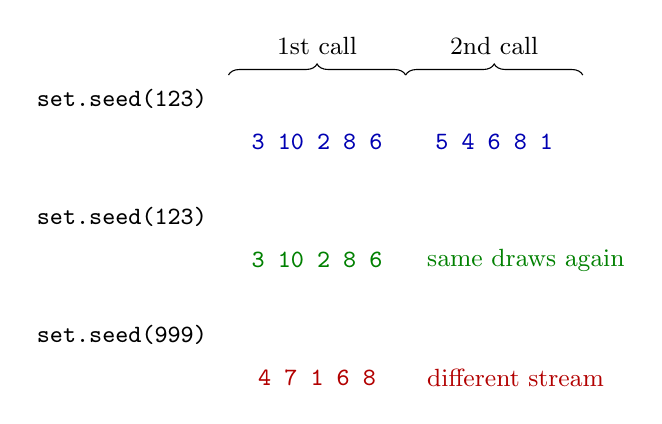
\begin{tikzpicture}[font=\small, >={Latex[length=2mm]}]
  % first run
  \node[anchor=east] at (-0.15,0.2) {\texttt{set.seed(123)}};
  \stream{0}{blue!12}{blue!70!black}
  \draw[decorate, decoration={brace, amplitude=4pt}] (0,0.5) -- node[above=4pt] {1st call} (2.25,0.5);
  \draw[decorate, decoration={brace, amplitude=4pt}] (2.25,0.5) -- node[above=4pt] {2nd call} (4.5,0.5);
  \node[blue!70!black] at (1.125,-0.35) {\texttt{3 10 2 8 6}};
  \node[blue!70!black] at (3.375,-0.35) {\texttt{5 4 6 8 1}};
  % second run, same seed
  \node[anchor=east] at (-0.15,-1.3) {\texttt{set.seed(123)}};
  \stream{-1.5}{blue!12}{blue!70!black}
  \node[green!50!black] at (1.125,-1.85) {\texttt{3 10 2 8 6}};
  \node[green!50!black, anchor=west] at (2.4,-1.85) {same draws again};
  % different seed
  \node[anchor=east] at (-0.15,-2.8) {\texttt{set.seed(999)}};
  \stream{-3.0}{red!12}{red!70!black}
  \node[red!70!black] at (1.125,-3.35) {\texttt{4 7 1 6 8}};
  \node[red!70!black, anchor=west] at (2.4,-3.35) {different stream};
\end{tikzpicture}
\end{document}
